% (c) 2012 -2014 Claudio Carboncini - claudio.carboncini@gmail.com
% (c) 2012 -2014 Dimitrios Vrettos - d.vrettos@gmail.com
\section{Esercizi}
\subsection{Esercizi dei singoli paragrafi}
\subsubsection*{\thechapter.1 - Espressioni letterali e valori numerici}
\begin{figure}[b]
\begin{minipage}[t]{.45\textwidth}
 \centering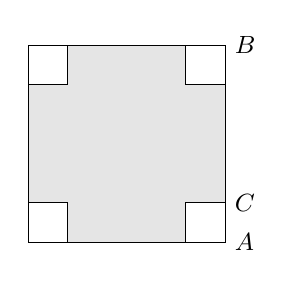
\begin{tikzpicture}[x=5mm, y=5mm,font=\small]
\definecolor{area}{gray}{0.9}
\draw [fill=area] (0,0) rectangle (5,5); 
\foreach \x in {0,4}{
\draw[fill=white] (\x,0) rectangle (\x+1,1);
\draw[fill=white] (\x,4) rectangle (\x+1,5);}
\node[right] at (5,0) {$A$};
\node [right] at (5,5) {$B$};
\node [right] at (5,1) {$C$};
\end{tikzpicture}
 \caption{Esercizio~\ref{ese:8.1}}\label{fig:8.1}
\end{minipage}
 \begin{minipage}[t]{.45\textwidth}
 \centering 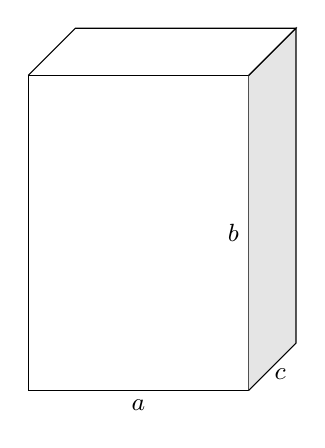
\begin{tikzpicture}[x=4mm, y=4mm,font=\small]
\definecolor{area}{gray}{0.9}
\draw(0,0) rectangle (7,10); 
\draw[fill=area, draw=black](7,0) -- (8.5,1.5)-- (8.5,11.5)--(7,10);
\draw(0,10) -- (1.5,11.5)-- (8.5,11.5)--(7,10);

\node[below] at (3.5,0) {$a$};
\node[left] at (7,5) {$b$};
\node[below] at (8,1) {$c$};
\end{tikzpicture}
 \caption{Esercizio~\ref{ese:8.10}}\label{fig:8.2}
\end{minipage}
\end{figure}

\begin{multicols}{2}
\begin{esercizio}
\label{ese:8.1}
Esprimi con una formula l'area della superficie della zona colorata di figura \ref{fig:8.1},
indicando con~$l$ la misura del lato~$AB$ e
con~$b$ la misura di~$AC$.

\emph{Svolgimento}: l'area del quadrato è \ldots\ldots,
l'area di ciascuno dei quadratini bianchi è \ldots\ldots. Pertanto l'area della
superficie in
grigio è \ldots\ldots
\end{esercizio}

\begin{esercizio}
\label{ese:8.2}
Scrivi l'espressione algebrica letterale relativa alla frase ``eleva al quadrato la differenza tra il cubo di un
numero e il doppio del suo quadrato''.

\emph{Svolgimento}: detto~$a$ il numero generico, il cubo di~$a$ si indica con \ldots,
il doppio del quadrato di~$a$ si indica con \ldots e infine
il quadrato della differenza sarà: \ldots
\end{esercizio}

\begin{esercizio}
\label{ese:8.3}
Traduci in parole della lingua italiana il seguente schema di calcolo:~$(a-b)^{3}$

\emph{Svolgimento}: ``Eleva al \ldots\ldots la differenza tra \ldots\ldots''
\end{esercizio}

\begin{esercizio}
 \label{ese:8.4}
Individua tra le espressioni letterali sottostanti, quelle scritte correttamente:
\begin{enumeratea}
\spazielenx
 \item $b\cdot {\frac{4}{5}}+\left(3-\frac{7}{2}\right)\cdot a-a$;
 \item $a\cdot 2-b^{4}$;
 \item $x\cdot (a-b)^{2}+(x-3)$;
 \item $x^{y}-a:2$;
 \item $-a+4b+c$;
 \item $\frac{a\cdot 1}{2}-\frac{a}{2}$.
\end{enumeratea}
\end{esercizio}
\end{multicols}

\begin{esercizio}
\label{ese:8.5}
 Collega con una freccia la proprietà dell'operazione con la sua scrittura attraverso lettere:
 \begin{multicols}{2}
 \noindent
 Commutativa dell'addizione\\
 Associativa della moltiplicazione\\
 Distributiva prodotto rispetto alla somma\\
 $a\cdot (x+y)=a\cdot x+a\cdot y$\\
 $\left(a\cdot b\right)\cdot c=a\cdot \left(b\cdot c\right)$\\
 ${a+b=b+a}$
 \end{multicols}
\end{esercizio}

\begin{esercizio}
\label{ese:8.6}
Esprimere con le lettere la proprietà commutativa della moltiplicazione

\emph{Svolgimento}: ``considerati~$a$ e~$b$ due numeri qualsiasi, la proprietà commutativa si esprime per mezzo dell'espressione \ldots\ldots; cioè \ldots\ldots\ldots''
\end{esercizio}

\begin{multicols}{2}
\begin{esercizio}
\label{ese:8.7}
Scrivi la formula che ci permette di calcolare l'area di un trapezio avente base maggiore~$B=5\unit{cm}$, base minore~$b=2\unit{cm}$ e altezza~$h=4\unit{cm}$.
\end{esercizio}

\begin{esercizio}
\label{ese:8.8}
Scrivi la formula che ci consente di calcolare il perimetro di un quadrato di misura~$l$.
\end{esercizio}

\begin{esercizio}
\label{ese:8.9}
Determina l'altezza~$h_i$ relativa all'ipotenusa~$BC$ del triangolo rettangolo~$ABC$.

Caso \emph{numerico}:~$\overline{AB}=8\unit{m}$, $\overline{AC}=15\unit{m}.$

Caso \emph{generale}: Indica con~$x$ e~$y$ le misure dei cateti, e determina la formula per calcolare la misura di~$h_i$.
\end{esercizio}

\begin{esercizio}
\label{ese:8.10}
Il volume della scatola di figura~\ref{fig:8.2} avente le dimensioni di~$7\unit{cm}$, $10\unit{cm}$, $2\unit{cm}$ è~$\ldots$

Generalizza la questione indicando con~$a$, $b$, $c$ la misura delle sue dimensioni \ldots\ldots

Se raddoppiamo ciascuna dimensione allora il volume diventa
 \begin{enumeratea}
 \item $2abc$;
 \item $a^{2}b^{2}c^{2}$;
 \item $6abc$;
 \item $8abc$.
 \end{enumeratea}
\end{esercizio}

\begin{esercizio}[\Ast]
\label{ese:8.11}
Scrivi sotto forma di espressioni letterali le seguenti frasi:
 \begin{enumeratea}
 \item moltiplica~$a$ per l'inverso di~$a$;
 \item sottrai ad~$a$ l'inverso di~$b$;
 \item sottrai il doppio di~$a$ al cubo di~$a$.
 \end{enumeratea}
\end{esercizio}

\begin{esercizio}
\label{ese:8.12}
Scrivi sotto forma di espressioni letterali le seguenti frasi:
 \begin{enumeratea}
 \item moltiplica~$a$ per l'opposto del cubo di~$a$:
 \item somma al triplo di~$a$ il doppio del quadrato di~$b$;
 \item moltiplica l'inverso di~$b$ per il quadrato dell'inverso di~$a$;
 \item somma al cubo di~$a$ il quadrato della somma di~$a$ e~$b$;
 \item dividi il quadrato di~$a$ per il triplo del cubo di~$b$;
 \item moltiplica il quadrato di~$b$ per l'inverso del cubo di~$a$;
 \item il cubo di un numero, aumentato di~2, è uguale al quadrato della differenza tra lo stesso numero e uno;
 \item il reciproco della somma dei quadrati di~$a$ e di~$b$;
 \item il cubo della differenza tra~1 e il cubo di~$a$;
 \item la somma dei quadrati di~$a$ e di~$b$ per il quadrato della differenza tra~$a$ e~$b$.
 \end{enumeratea}
\end{esercizio}
\end{multicols}
\subsubsection*{\thechapter.2 - Il valore numerico di un'espressione letterale}

\begin{esercizio}
\label{ese:8.13}
Consideriamo l'espressione letterale~$E=-3a+2(-a+1)$.

Osserviamo che vi compare una sola variabile, la lettera~$a$; supponiamo che~$E$ rappresenti uno schema di calcolo tra
numeri interi relativi. Determiniamo il valore dell'espressione per alcuni valori della variabile:
\begin{align*}
a =-2 & \quad\Rightarrow\quad E =-3\cdot (-2)+2\cdot (-(-2)+1) =6+2\cdot (2+1) =6+6 =12 \\
a =+1 & \quad\Rightarrow\quad E =-3\cdot (1)+2\cdot(-(1)+1) =-3+2\cdot (-1+1) =-3+0 =-3 \\
a =-1 & \quad\Rightarrow\quad E =-3\cdot (\ldots)+2\cdot (\ldots +1) =\ldots \ldots \ldots
\end{align*}

Completa la seguente tabella.

 \begin{tabular*}{.9\textwidth}{@{\extracolsep{\fill}}*{9}{c}}
 \toprule
 $a$ & $-2$ & $1$ & $-1$ & $0,1$ & $\dfrac{4}{5}$ & $-\dfrac{7}{5}$ & $-11$ &$0$\vspace{1.05ex}\\
 \midrule
 $E=-3a+2(-a+1)$& $12$ & $-3$ &	& & & & &\\
 \bottomrule
 \end{tabular*}
\end{esercizio}
\pagebreak
\begin{esercizio}[\Ast]
\label{ese:8.14}
Calcola il valore dell'espressione letterale $E=\dfrac{3}{7}ab-\dfrac{1}{2}(a-b)+a-b$ le cui variabili~$a$, $b$ rappresentano numeri razionali, per i valori assegnati nella tabella sottostante.

\emph{Svolgimento}: se vogliamo calcolare il valore dell'espressione letterale dobbiamo scegliere due numeri razionali, uno da
assegnare alla variabile~$a$, l'altro alla variabile~$b$.

\begin{tabular*}{.9\textwidth}{@{\extracolsep{\fill}}*{5}{c}}
 \toprule
 $a$ & $3$ & $0$ & $2$ & $-\dfrac{3}{2}$\vspace{1.05ex}\\
 $b$ & $-3$ & $-\dfrac{1}{2}$ & $0$ & $-\dfrac{3}{2}$ \\
 \midrule
 $E=\dfrac{3}{7} ab-\dfrac{1}{2}(a-b)+a-b$& & & &\\
 \bottomrule
 \end{tabular*}
\end{esercizio}

\begin{esercizio}
\label{ese:8.15}
Calcolare il valore numerico dell'espressione:~$\dfrac{a}{a-3}+\dfrac{b}{3-b}$ per~$a = -1$, $b = 0$.

\emph{Svolgimento}:~$\dfrac{-1}{-1-3}+\dfrac{0}{3-0}= \ldots\ldots$
\end{esercizio}

\begin{esercizio}
\label{ese:8.16}
Calcola il valore dell'espressione~$E=\dfrac{x-y}{3x}$ costruita con le variabili~$x$ e~$y$ che rappresentano
numeri razionali. L'espressione letterale assegnata traduce il seguente schema di calcolo: ``la divisione tra la
differenza di due numeri e il triplo del primo numero''. Completa la seguente tabella:

 \begin{tabular*}{.9\textwidth}{@{\extracolsep{\fill}}*{7}{c}}
 \toprule
 $x$ & $\dfrac{3}{4}$ & $\dfrac{19}{3}$ & $\dfrac{3}{4}$ & $-4$ & $\ldots$ & $\ldots$ \vspace{1.05ex}\\
 $y$ & $-\dfrac{1}{2}$ & $0$ & $0$ & $-2$ & $\ldots$ & $\ldots$ \\
 \midrule
 $E=\dfrac{x-y}{3x}$& & & & & &\\
 \bottomrule
 \end{tabular*}

Ti sarai accorto che in alcune caselle compare lo stesso valore per~$E$: perché secondo te succede questo fatto?

Vi sono, secondo te, altre coppie che fanno assumere ad~$E$ quello stesso valore?

\end{esercizio}


\begin{esercizio}[\Ast]
\label{ese:8.17}
Scrivi con una frase le seguenti espressioni
\begin{multicols}{2}
 \begin{enumeratea}
\spazielenx
 \item $3a$;
 \item $\dfrac{2a}{3b^{2}}$.
 \end{enumeratea}
\end{multicols}
\end{esercizio}

\begin{esercizio}
\label{ese:8.18}
Scrivi con una frase le seguenti espressioni
\begin{multicols}{4}
 \begin{enumeratea}
\spazielenx
 \item $2b-5a$;
 \item $a {\dfrac{1}{a}}$;
 \item $(a+b)^{2}$;
 \item $\dfrac{3x+y}{2x^{2}}$.
 \end{enumeratea}
\end{multicols}
\end{esercizio}
\pagebreak
\begin{esercizio}
\label{ese:8.19}
Completa la tabella sostituendo nell'espressione della prima colonna i valori indicati.

 \begin{tabular*}{.93\textwidth}{l@{\extracolsep{\fill}}*{8}{c}}
 \toprule
 Espressione & $x=1$ & $x=-1$ & $x=0$ & $x=2$ & $x=\dfrac{1}{2}$ & $x=-\dfrac{1}{2}$ & $x=0,1$ & $x=\dfrac{1}{10}$\\
 \midrule
 $2x+1$ & & & & & & & &\\
 $-(3x-2)$ & & & & & & & &\\
 $x^{2}+2x+2$ & & & & & & & &\\
 $x^{2}-x$ & & & & & & & &\\
 $-x^{2}+x-1$ & & & & & & & &\\
 $x^{3}-1$ & & & & & & & &\\
 $x^{3}+3x^{2}$ & & & & & & & &\\
 $-x^{3}+x^{2}-x$ & & & & & & & &\\
 $-(x+1)^{2}$ & & & & & & & &\\
 $\dfrac{x+1}{1-x}$ & & & & & & & &\\
 \bottomrule
 \end{tabular*}
\end{esercizio}

\begin{esercizio}
\label{ese:8.20}
Calcola il valore numerico delle seguenti espressioni algebriche:
 \begin{enumeratea}
\spazielenx
 \item $3x^{2}-\dfrac{1}{4}x^{2}\quad$ per~$x=\dfrac{1}{2}\quad$ \emph{Svolgimento}:~$3\cdot \left(\dfrac{1}{2}\right)^{2}-\dfrac{1}{4}\cdot \left(\dfrac{1}{2}\right)^{2}=\ldots \ldots \ldots =\dfrac{11}{16}$;
 \item $5a^{2}b\quad$ per~$a=-{\dfrac{1}{2}}$, $b=\dfrac{3}{5}\quad$ \emph{Svolgimento}:~$5\cdot \left(-{\dfrac{1}{2}}\right)^{2}\cdot \left(\dfrac{3}{5}\right)=\ldots \ldots \ldots \ldots $;
 \item $\dfrac{3}{2}\cdot a^{2}+\dfrac{1}{2}a-1\quad$ per~$a=0$, per~$a=-1$ e~$a=2$;
 \item $2\cdot x^{5}-8\cdot x^{4}+3\cdot x^{3}+2\cdot x^{2}-7\cdot x+8\quad$ per~$x=+1$ e~$x=-1$.
 \end{enumeratea}
\end{esercizio}

\begin{esercizio}
\label{ese:8.21}
Calcola il valore numerico delle seguenti espressioni algebriche:
 \begin{enumeratea}
\spazielenx
 \item $(x-1)\cdot (x-2)\cdot (x+3)\quad$ per~$x=0$, $x= -1$ e~$x= 2$;
 \item $x^{2}+2x+1\quad$ per~$x=0$, $x= -1$ e~$x= 1$;
 \item $-a^{2}\cdot b\cdot c^{3}\quad$ per~$a=1$, $b=-1$, $c=-2$ e~$a=-1$, $b=\dfrac{9}{16}$, $c=\dfrac{4}{3}$;
 \item $-{\dfrac{3}{2}}a+2b^{2}+11\quad$ per~$a=-20$, $b=-{\dfrac{1}{2}}$ e~$a=\dfrac{2}{3}$, $b=0$;
 \item $-a^{2}+\dfrac{1}{a}-3\cdot a^{3}\quad$ per~$a=\dfrac{1}{3}$, $a=-1$ e~$a=+1$.
 \end{enumeratea}
\end{esercizio}

\begin{esercizio}[\Ast]
\label{ese:8.22}
Calcola il valore numerico delle seguenti espressioni algebriche:
 \begin{enumeratea}
\spazielenx
 \item $4a+a^{3}\quad$ per~$a=2$ e~$a=1$;
 \item $2a+5a^{2}\quad$ per~$a=-1$ e~$a=0$;
 \item $3x+2y^{2}(xy)\quad$ per~$x=1$, $y=-{\dfrac{1}{2}}$ e~$x=\dfrac{1}{3}$, $y=-1$;
 \item $a^{2}-b^{-1}+ab\quad$ per~$a=1$, $b=\dfrac{1}{2}$ e~$a=0$, $b=-1$;
 \item $3a^{2}b-7ab+a\quad$ per~$a=1$, $b=3$ e~$a=-1$, $b=-3$.
 \end{enumeratea}
\end{esercizio}
\pagebreak
\begin{esercizio}[\Ast]
\label{ese:8.23}
Calcola il valore numerico delle seguenti espressioni algebriche:
 \begin{enumeratea}
\spazielenx
 \item $3xy-2x^{2}+3y^{2}\quad$ per~$x=\dfrac{1}{2}$, $y=2$ e~$x=2$, $y=\dfrac{1}{2}$;
 \item $\dfrac{2}{3}a\left(a^2-b^2 \right) \quad$ per~$a=-3$, $b=-1$ e~$a=\dfrac{1}{3}$, $b=0$;
 \item $\dfrac{xy}{x}+3xy^{3}\quad$ per~$x=2$, $y=-1$ e~$x=-2$, $y=+1$;
 \item $\dfrac{1}{2}\dfrac{(a+b)^{2}}{a^{2}b^{2}}+2a+3b\quad$ per~$a=\dfrac{1}{4}$, $b=-2$ e $a=\dfrac{1}{2}$, $b=-{\dfrac{1}{2}}$;
 \item $3x^{3}+2xy\left(\dfrac{x^{2}}{y}\right)+2y^{2}\quad$ per~$x=-2$, $y=\dfrac{3}{4}$ e~$x=-1$, $y=-1$.
 \end{enumeratea}
\end{esercizio}

\begin{esercizio}[\Ast]
\label{ese:8.24}
Calcola il valore numerico delle seguenti espressioni algebriche:
 \begin{enumeratea}
\spazielenx
 \item $\dfrac{4a-7b}{(2a+3b)^{3}}\cdot ab^{3}\quad$ per~$a=-{\dfrac{1}{2}}$, $b=1$ e~$a=-{\dfrac{1}{4}}$, $b=\dfrac{2}{3}$;
 \item $\dfrac{4x^{2}-5xy+3y}{6x+y^{2}}\quad$ per~$x=-1$, $y=2$ e~$x=0$, $y=-2$;
 \item $\dfrac{x}{x+3}+y^{2}-\dfrac{xy-3x+y}{(\mathit{xy})^{2}}\quad$ per~$x=3$, $y=\dfrac{1}{3}$ e~$x=1$, $y=-1$;
 \item $\dfrac{(4a-2b)\cdot {2a^{2}}}{3b^{3}}\cdot {\dfrac{3}{4}}ab+a^{3}\quad$ per~$a=1$, $b=-1$ e~$a=0$, $b=-3$.
 \end{enumeratea}
\end{esercizio}

\subsubsection*{\thechapter.3 - Condizione di esistenza di un'espressione letterale}

\begin{esercizio}
 \label{ese:8.25}
Se~$E=-{\dfrac{x-2}{2}x^{2}}$ completa la tabella:
\begin{center}
\begin{tabular*}{.4\textwidth}{l@{\extracolsep{\fill}}*{4}{c}}
\toprule
$x$ & 2 & 0 & $\dfrac{3}{4}$ & $-{\dfrac{5}{8}}$\\
E & & & & \\
\bottomrule
\end{tabular*}
\end{center}
\end{esercizio}

\begin{esercizio}
 \label{ese:8.26}
Calcola il valore numerico dell'espressione:~$\dfrac{3x-1}{x}$ per~$x = 0$.

\emph{Svolgimento}: Sostituendo alla~$x$ il valore assegnato si ha una
divisione per \ldots e quindi \dotfill
\end{esercizio}

\begin{esercizio}[\Ast]
 \label{ese:8.27}
Sostituendo alle lettere i numeri a fianco indicati, stabilisci se le
seguenti espressioni hanno significato:
\TabPositions{8cm}
\begin{enumeratea}
\item $\dfrac{x+3}{x}$\quad per~$x=0$ \tab\boxSi\quad\boxNo
\item $\dfrac{x^{2}+y}{x}$\quad per~$x=3$, $y=0.$ \tab\boxSi\quad\boxNo
\item $\dfrac{(a+b)^{2}}{(a-b)^{2}}$\quad per~$a=1$, $b=1$ \tab\boxSi\quad\boxNo
\item $\dfrac{5x^{2}+3y-xy}{(x^{2}+y)^{3}}$\quad per~$x=2$, $y=-2$ \tab\boxSi\quad\boxNo
\item $\dfrac{a^{3}+b+6a^{2}}{a^{2}+b^{2}+3ab-3a^{2}}$\quad per~$a=1$, $b=\dfrac{4}{3}$ \tab\boxSi\quad\boxNo
\end{enumeratea}
\end{esercizio}

\begin{esercizio}
 \label{ese:8.28}
 Sostituendo alle lettere numeri razionali
arbitrari, determina se le seguenti uguaglianze tra formule sono
vere o false
\TabPositions{8cm}
\begin{enumeratea}
 \item $a^{2}+b^{2}=(a+b)^{2}$ \tab\boxV\quad\boxF
 \item $(a-b)\cdot (a^{2}+a\cdot b+b^{2})=a^{3}-b^{3}$ \tab\boxV\quad\boxF
 \item $(5a-3b)\cdot (a+b)=5a^{2}+ab-3b^{2}$ \tab\boxV\quad\boxF
\end{enumeratea}
\end{esercizio}

\begin{esercizio}
 \label{ese:8.29}
 Se~$n$ è un qualunque numero naturale,
l'espressione~$2\cdot n+1$ dà origine:
\begin{multicols}{2}
\boxA\quad ad un numero primo

\boxB\quad ad un numero dispari

\boxC\quad ad un quadrato perfetto

\boxD\quad ad un numero divisibile per~3
\end{multicols}
\end{esercizio}

\begin{esercizio}
 \label{ese:8.30}
 Quale formula rappresenta un multiplo di~5,
qualunque sia il numero naturale attribuito ad~$n$?
\begin{center}
 \boxA\quad~$5+n$ \quad\boxB\quad~$n^{5}$ \quad\boxC\quad~$5\cdot n$ \quad\boxD\quad~$\dfrac{n}{5}$
\end{center}
\end{esercizio}

\begin{esercizio}
 \label{ese:8.31}
 La tabella mostra i valori assunti da~$y$ al variare di~$x$. Quale delle seguenti è
la relazione tra~$x$ e~$y$?

\begin{center}
\begin{tabular*}{.4\textwidth}{l@{\extracolsep{\fill}}*{4}{c}}
\toprule
$x$ & 1 & 2 & 3 & 4\\
$y$ & 0 & 3 & 8 & 15\\
\bottomrule
\end{tabular*}

 \vspace{1.10ex}\boxA\quad~$y=x+1$ \quad\boxB\quad~$y=x^{2}-1$ \quad\boxC\quad~$y=2x-1$ \quad\boxD\quad~$y=2x^{2}-1$
\end{center}
\end{esercizio}

\begin{esercizio}
 \label{ese:8.32}
 Verifica che sommando tre numeri dispari consecutivi si ottiene un
multiplo di~3. Utilizza terne di numeri dispari che iniziano per~3;
7; 11; 15; 21. Per esempio~$3+5+7= \ldots$ multiplo di 3? Vero. Continua tu.
\end{esercizio}

\subsection{Risposte}
\begin{multicols}{2}
\paragraph{\thechapter.11.}
a)~$a \cdot\frac{1}{a}$,\quad b)~$a-\frac{1}{b}$,\quad c)~$a^3-2a$.
\paragraph{\thechapter.14.} $a=3$; $b=-3\rightarrow -\frac{6}{7}$,\quad~$a=0$; $b=-\frac{1}{2}\rightarrow \frac{1}{4}$,\quad~$a=-\frac{3}{2}$; $b=-\frac{3}{2}\rightarrow -\frac{27}{28}$.
\paragraph{\thechapter.17.}
a)~ Il triplo di~$a$,\quad ~b)~Dividi il doppio di~$a$ per il triplo del quadrato di~$b$.
\paragraph{\thechapter.22.}
a)~$a=2 \rightarrow~16$; $a=1 \rightarrow~5$, \quad b)~$a=-1 \rightarrow~3$; $a=0 \rightarrow~0$,
c)~$x=1$; $y=-\frac{1}{2} \rightarrow \frac{11}{4}$,\quad d)~$a=1$; $b=\frac{1}{2}\rightarrow -\frac{1}{2}$, \quad e)~$a=1$; $b=3 \rightarrow -11$.
\paragraph{\thechapter.23.}
a)~$x=\frac{1}{2}$; $y=2 \rightarrow \frac{29}{2}$, \quad b)~$a=-3$; $b=-1 \rightarrow -16$, \quad c)~$x=2$,$y=-1 \rightarrow -7$,
d)~$a=\frac{1}{4}$; $b=-2 \rightarrow \frac{5}{8}$,\quad e)~$x=-2$; $y=\frac{3}{4} \rightarrow -\frac{311}8{}$,\quad
\paragraph{\thechapter.24.}
a)~$a=-\frac{1}{2}$; $b=1 \rightarrow \frac{9}{16}$,
b)~$x=-1$; $y=2 \rightarrow -10$,\quad c)~$x=3$; $y=\frac{1}{3} \rightarrow \frac{149}{18}$,\quad d)~$a=1$; $b=-1 \rightarrow~4$.
\paragraph{\thechapter.27.} Non ha significato perché $\frac{4}{0}$ non è un numero.
\end{multicols}
